\documentclass{article}
\usepackage[utf8]{inputenc}
\usepackage{physics}
\usepackage{amsmath}
\usepackage{geometry}

 \geometry{
 a4paper,
 total={170mm,257mm},
 left=20mm,
 top=20mm,
 }
\usepackage{ amsfonts }

\usepackage{natbib}
\usepackage{graphicx}
\usepackage{ amssymb}
\usepackage[utf8]{inputenc}

\title{Metodos computaiconales: Tarea 4
}

\author{ Juan Pablo Acuña Acosta
}
\date{November 2018}


\begin{document}

\maketitle

\section{ODE}

Resulatados Ecuacion diferencial ordinaria\\

\begin{figure}[h]
  \centering
  \begin{minipage}[b]{0.5\textwidth}
    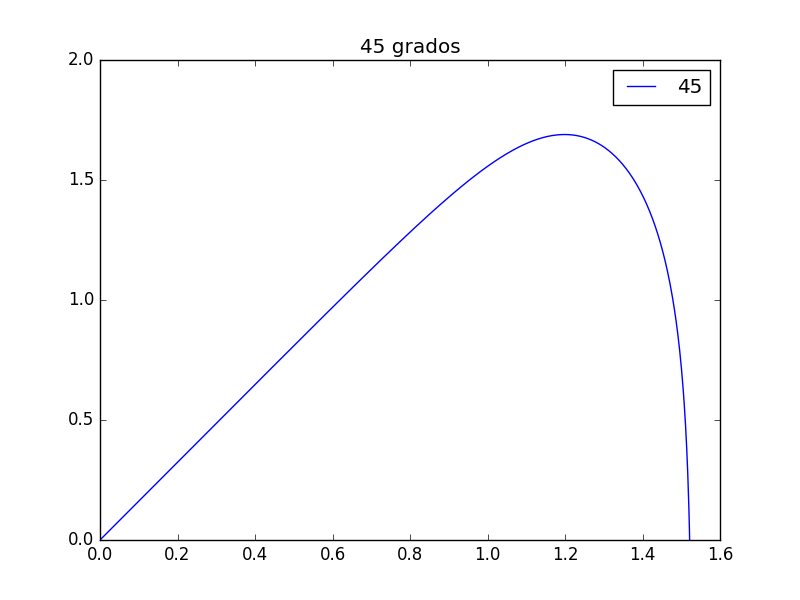
\includegraphics[width=\textwidth]{45.png}
    \caption{Proyectil para 45 grados}
  \end{minipage}
  \hfill
  \begin{minipage}[b]{0.5\textwidth}
    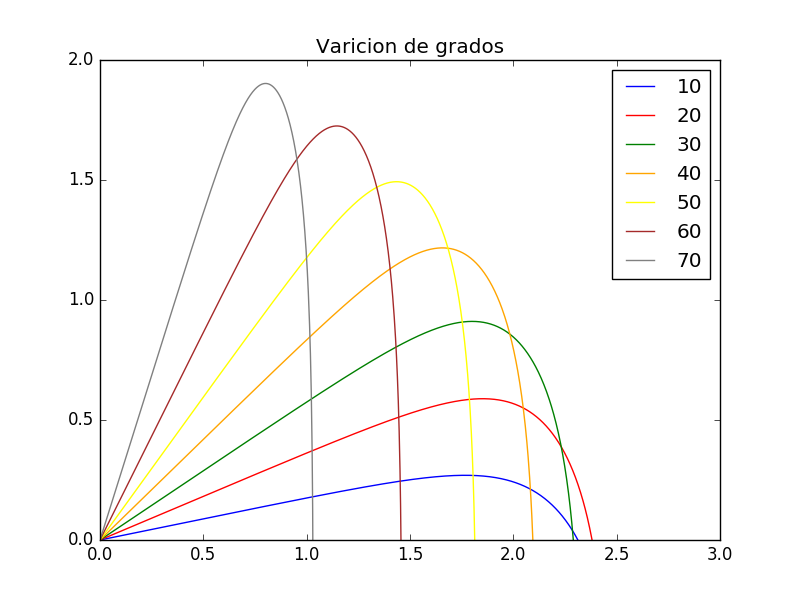
\includegraphics[width=\textwidth]{variosAngulos.png}
    \caption{Grafica para varios angulos}
  \end{minipage}
\end{figure}


Se observa que para el angulo de 45 grados las distancia pobtenida no es la mayor como se esperaba sino la mayor distancia se da con el angulo de 20 grados.\\





\section{PDE}
\begin{figure}[h]
\centering
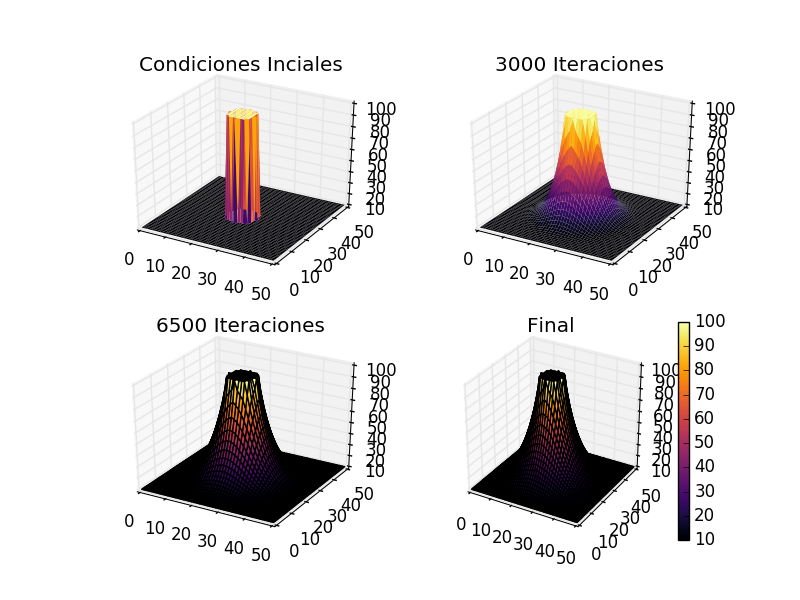
\includegraphics[scale=0.9]{Normales.png}
\caption{Fronteras a 10 grados}
\label{fig:universe}
\end{figure}
Para fronteras fija se observa que la superficie que representa la temperatura aumenta de manera uniforme. Se logra ver que al final obtiene un "cono" sin punta.

\begin{figure}[h]
\centering
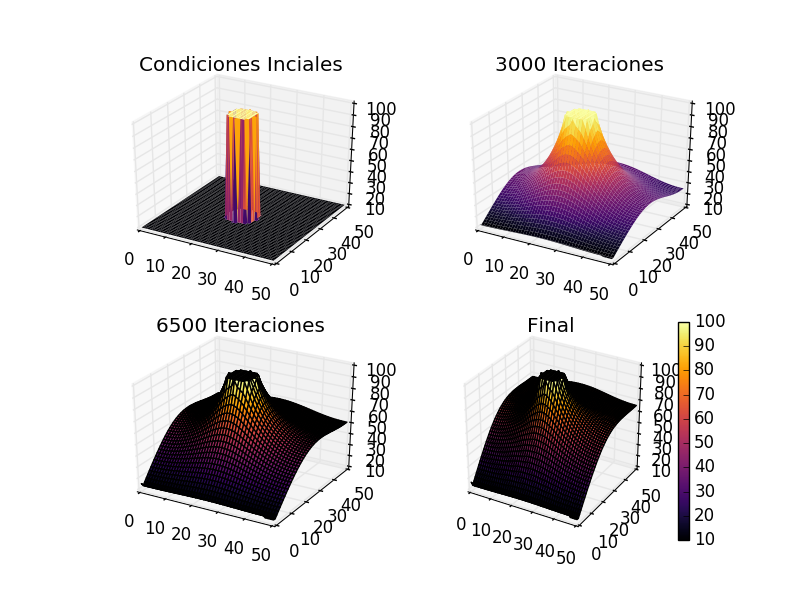
\includegraphics[scale=0.9]{Abiertas.png}
\caption{Fronteras abiertas}
\label{fig:universe}
\end{figure}
Para fronteras abiertas, se observa que las fronteras poco a poco van subiendo de temperatura,y las esquinas se demoran mas en suubir de temperatura debido a que estan mas alejadas de la fuente caliente. \\

\begin{figure}[h]
\centering
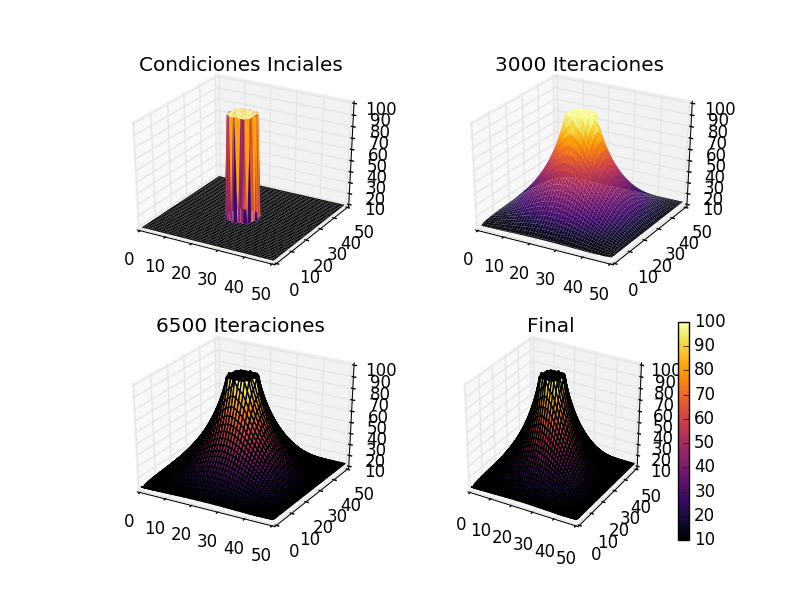
\includegraphics[scale=0.9]{Periodicas.png}
\caption{Fronteras Periodicas}
\label{fig:universe}
\end{figure}
Para fronteras periodicas se observa un comportamiento muy similar a fronteras abiertas. 




\end{document}

